\documentclass{standalone}
\usepackage{tikz}
\usepackage{amsmath}

\usetikzlibrary{arrows.meta,decorations.pathreplacing}

\tikzset{
    line/.style={
        thick
    },
    arrow/.style={
        line,
        ->,
        > = {
            Triangle[length=2.0mm, width=2.0mm]
        }
    }
}

% Switch to Sans Serif font.
\renewcommand{\familydefault}{\sfdefault}

\renewcommand{\wedge}{$\vphantom{\big|}$}


\begin{document}
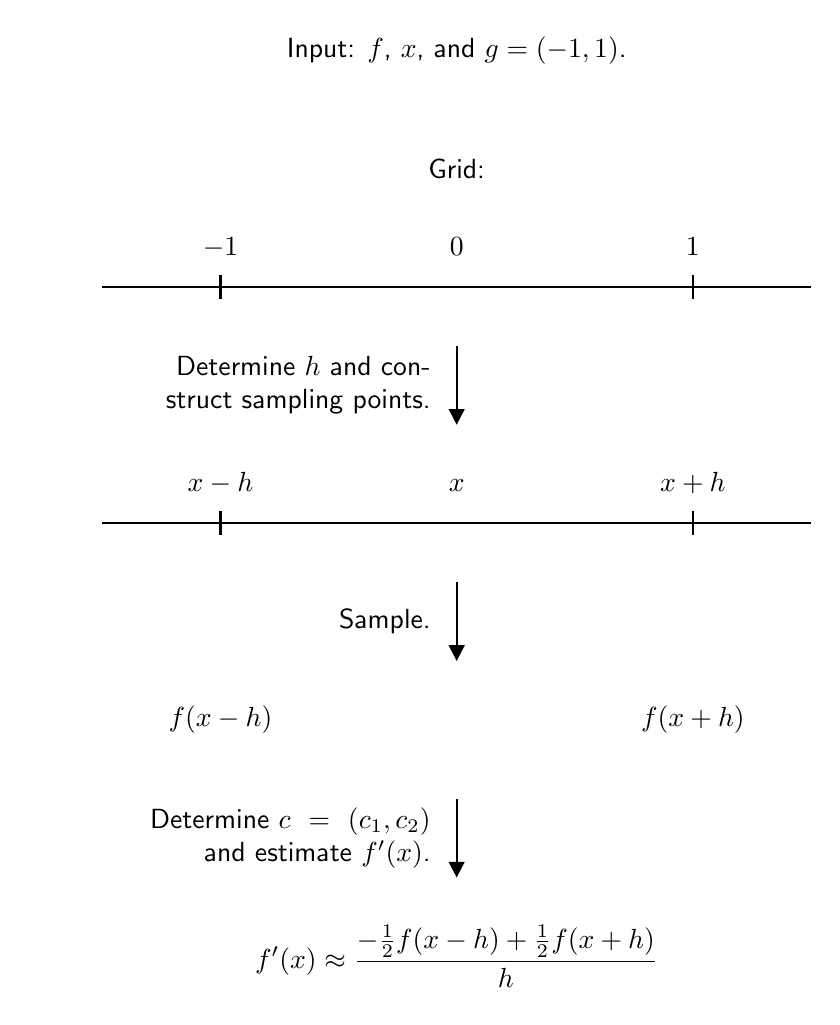
\begin{tikzpicture}[xscale=3]
    % Grid:
    \begin{scope}[shift={(0, 6)}]
        \node () at (0, 0) {Input: $f$, $x$, and $g=(-1,1)$.};
        \node () at (0, -1.5) {Grid:};
    \end{scope}
    % Grid:
    \begin{scope}[shift={(0, 3)}]
        \draw [line] (-1.5, 0) -- (1.5, 0);
        \draw [line] (-1, -0.15) --
            % node [pos=0, anchor=north] {$\wedge g_1$}
            node [pos=1, anchor=south] {$\wedge -1$} (-1, 0.15);
        \draw [line] (1, -0.15) --
            % node [pos=0, anchor=north] {$\wedge g_2$}
            node [pos=1, anchor=south] {$\wedge 1$} (1, 0.15);
        \path [] (0, -0.15) -- node [pos=1, anchor=south] {$\wedge 0$} (0, 0.15);
        \draw [arrow] (0, -.75) -- node [pos=0.5, anchor=east, xshift=-2mm, text width=4.5cm, align=right] {Determine $h$ and construct sampling points.} (0, -1.75);
    \end{scope}
    % Sampling points:
    \begin{scope}
        \draw [line] (-1.5, 0) -- (1.5, 0);
        \draw [line] (-1, -0.15) --
            % node [pos=0, anchor=north] {$\wedge x_{1}$}
            node [pos=1, anchor=south] {$\wedge x - h$} (-1, 0.15);
        \draw [line] (1, -0.15) --
            % node [pos=0, anchor=north] {$\wedge x_{2}$}
            node [pos=1, anchor=south] {$\wedge x + h$} (1, 0.15);
        \path [] (0, -0.15) -- node [pos=1, anchor=south] {$\wedge x$} (0, 0.15);
        \draw [arrow] (0, -.75) -- node [pos=0.5, anchor=east, xshift=-2mm, text width=5cm, align=right] {Sample.} (0, -1.75);
    \end{scope}
    % Sample:
    \begin{scope}[shift={(0, -2.5)}]
        \node () at (-1, 0) {$f(x - h)$};
        \node () at (1, 0) {$f(x + h)$};
        \draw [arrow] (0, -1) -- node [pos=0.5, anchor=east, xshift=-2mm, text width=4.5cm, align=right] {Determine $c=(c_1,c_2)$ and estimate $f'(x)$.} (0, -2);
    \end{scope}
    % Estimate:
    \begin{scope}[shift={(0, -5.5)}]
        \node () at (0, 0) {$\displaystyle f'(x) \approx \frac{-\frac{1}{2}f(x - h) + \frac{1}{2} f(x + h)}{h}$};
    \end{scope}
\end{tikzpicture}
\end{document}